\chapter{Background}
\label{ch:bg}
In this chapter, we discuss background information and related work for Facet Web Search, an extension of faceted search in the open-domain web setting. Faceted search is a heavily interdisciplinary area, where different aspects of information retrieval, knowledge representation, human computer interaction must be considered all together. Therefore, we first describe related topics in these areas as a background for faceted search/Faceted Web Search. Then, we describe faceted search, Faceted Web Search and previous research on these topics. After that, we discuss related approaches that aim to achieve the same goals as our work. We defer discussion of some related work to later chapters where the context makes it more appropriate.

\section{Knowledge Representation}
Faceted search is built upon taxonomy and faceted taxonomy, which are two types of knowledge representations that haven been studied for a long history.

\subsection{Taxonomy}
\label{sec:bg-taxonomy}
The word \concept{taxonomy} was originally referred to the classification of biological organisms. Its history dates back to more than two millennia ago. At that time, the Greek philosopher Aristotle first classified all living things into a hierarchical classification system, a taxonomy~\cite{tunkelang2009faceted}. The taxonomy classifies living things by dividing them into two groups, plants and animals; further dividing animals into those ``red blood'' and ``no red blood''; those with no red blood into ``hard bodies'' and ``soft bodies''; and so forth (Figure~\ref{fig:bg-aristotle}).
\begin{figure}[!htbp]
\centering
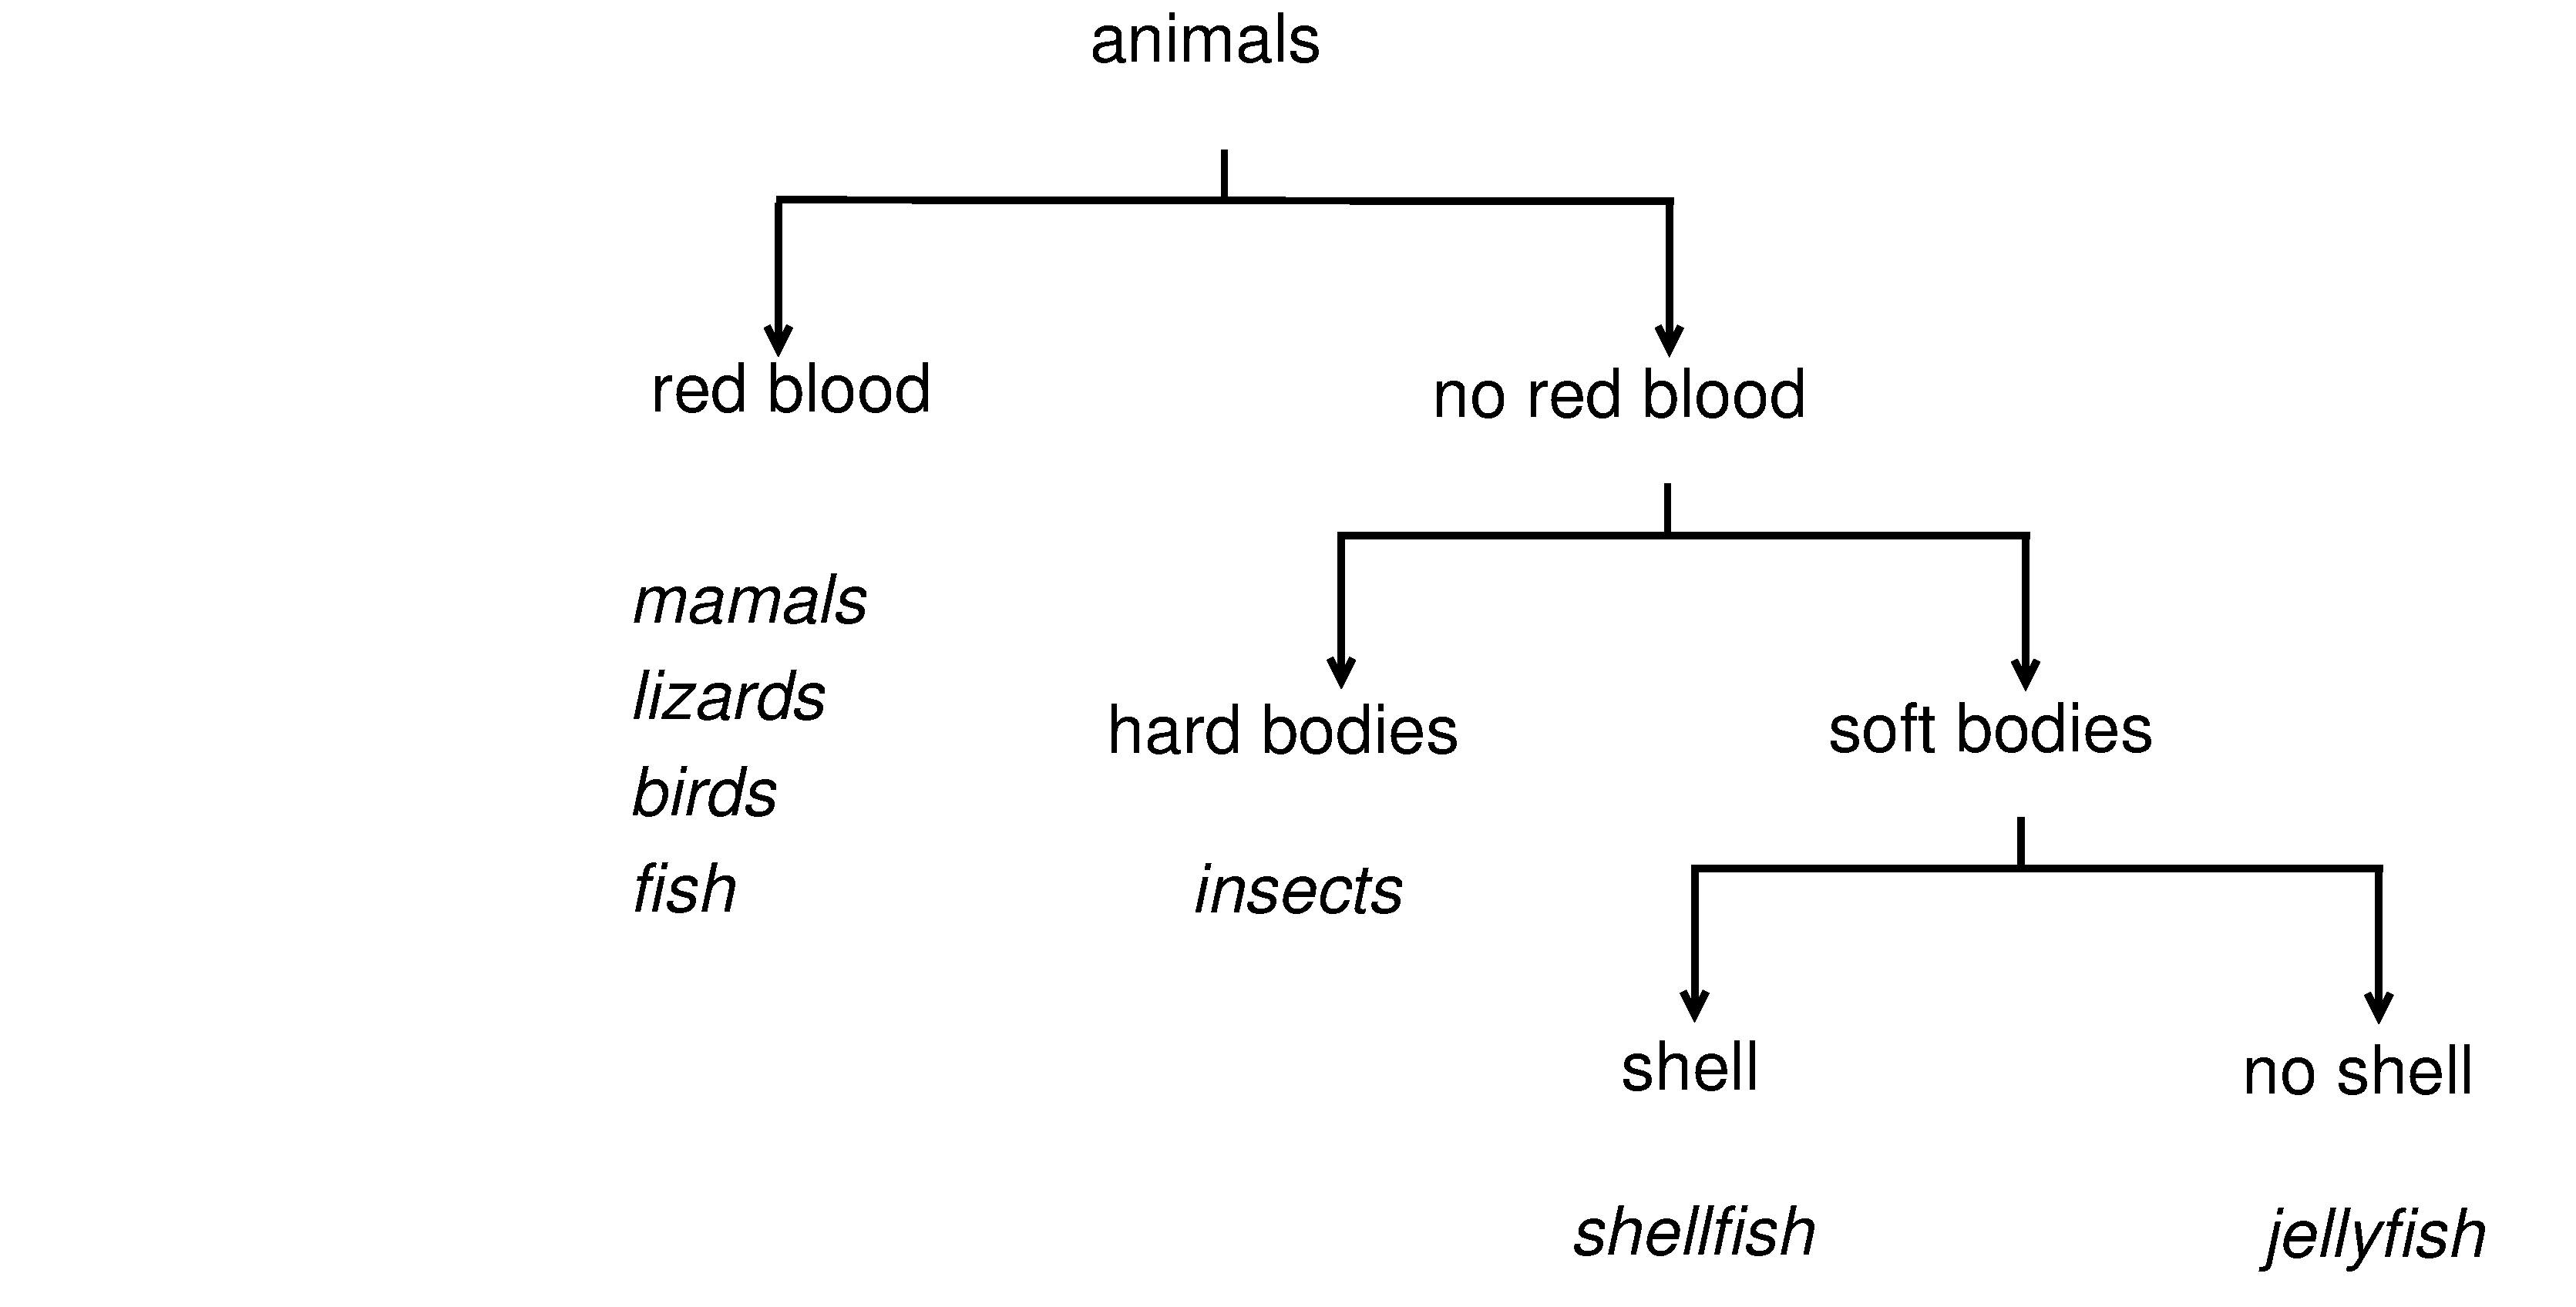
\includegraphics[width=0.8\columnwidth]{drawing/aristotle.eps}
\caption{A subset of Aristotle's knowledge taxonomy~\cite{tunkelang2009faceted}}
\label{fig:bg-aristotle}
\end{figure}

Today, the word \concept{taxonomy} refers more generally to any hierarchical classification schema. \citet{tunkelang2009faceted} described a taxonomy as an organization of things or abstractions into a hierarchy or tree structure. Similarly, \citet{sacco2009dynamic} described a taxonomy as a concept hierarchy going from the most general to the most specific concepts, into which information objects can be classified. Using the Aristotle's taxonomy as an example, we can see that concepts or abstractions of animals are organized in a tree. The root node \concept{animals} corresponds to the set of all animals. Its children represent the top-level divisions of the animals, one representing \concept{red blood} animals and one representing \concept{no red blood} animals. Their children correspond to the subdivisions of those animals; and so forth. Information objects are classified directly into concepts in the tree. For example, the object \concept{jellyfish} is classified to the concept \concept{no shell} and the 
object \concept{insects} is classified to the concept \concept{hard bodies}. 

To provide a more clear definition for a taxonomy, we synthesize its previous definitions and formulations~\cite{sacco2009dynamic, tzitzikas2005compound}, and define a taxonomy as follows:
\begin{definition}
\label{def:taxonomy}
A \textbf{taxonomy} is a tree of concepts with all concepts subsuming their descendant concepts.
\end{definition}
\noindent Next we explain the terminology used in this definition. First, informally, a \textbf{tree} (, like a real but upside-down tree,) has one single root node at the top, leaf nodes at the bottom, and branches connecting each nonleaf parent node to its children. (See \citet{garnier2009discrete} for a formal definition of a tree.) Figure~\ref{fig:bg-aristotle} shows an example of tree. The root node is \concept{animals}, and the parent nodes have edges pointing to their children. \textbf{Descendants} of a node $A$ are nodes under $A$'s branch. For example, Descendants of \concept{no red blood} include \concept{hard bodies}, \concept{soft bodies}, \concept{shell} and \concept{no shell}. A tree of concepts are simply a tree using concepts as nodes.

Second, a \textbf{concept} in a taxonomy is an abstraction which identifies all the information objects classified under it (including the information objects that are classified to its descendants in the concept tree). For example, in Figure~\ref{fig:bg-aristotle}, the concept \concept{no red blood} identifies all ``no-red-blood'' animals in the taxonomy, including \concept{inserts}, \concept{shellfish}, \concept{jellyfish} classified to its descendants. More formally, a \textbf{concept} $C$ can be defined as a set of information objects $C=\{d\}$. However, before being materialized with information objects, a concept is just an abstraction for a set of potential information objects. Also, concepts are often presented by their textual labels to convey the concept meaning to users.

Last, in the definition, the concept tree is constrained by having concepts in the tree subsumes all its descendant concepts. A concept $A$ is \textbf{subsumed} by a concept $B$ ($A \preccurlyeq B$) if the set of information objects classified under $A$ is intensionally constrained to be equal to or a subset of the set of objects classified under $B$: $A \subseteq B$. For example, in Figure~\ref{fig:bg-aristotle}, we can say that the concept \concept{shell} is subsumed by the concept \concept{no red blood}, because every animals classified under \concept{shell} is also classified under \concept{no red blood}. This definition of subsumption indicates a reflexive and transitive binary relation over concepts. It is very general, and thus can model many different reflexive and transitive binary semantic relations, such as IS-A and PART-OF. For example, the subsumption relation \concept{shell} $\preccurlyeq$ \concept{no red bold} indicates a ``shell'' animal is a ``no-red-blood'' animal. For PART-OF relations, an 
example is a taxonomy of United States locations in which the concept \concept{USA} has a child node \concept{MA}, and the concept \concept{MA} has a child node \concept{Amherst}. Thus, we have \concept{MA} $\preccurlyeq$ \concept{USA},  \concept{Amherst} $\preccurlyeq$ \concept{MA} and \concept{Amherst} $\preccurlyeq$ \concept{USA} (from the transitive property). Here the subsumption relations between these locations model PART-OF relations (\eg, \concept{MA} is a part of \concept{USA}).



%Based on the definitions of concepts and subsumption, a taxonomy can be defined as a tree of concepts with the concepts subsuming all their descendant concepts, or more formally:
%\begin{definition}
%A \textbf{taxonomy} is a tree $(\mathcal{C}, E)$, where $\mathcal{C}=\{C\}$ is a set of concepts and the nodes in the tree. $E$ is the set of edges in the tree. For any $C\in\mathcal{C}$ and any $C'$ in $Descendant_E(C)$, $C' \preccurlyeq C$, where $Descendant_E(C)$ is the set of all descendant nodes of $C$ in the tree, and $\preccurlyeq$ is the subsumption relation.
%\end{definition} 
%\citet{tzitzikas2005compound} provided a formal definition for a taxonomy:
%\begin{definition}
% A \textbf{taxonomy} is a pair $(\mathcal{C}, \preccurlyeq)$, where $\mathcal{C}=\{C\}$ is a set of concepts, and $\preccurlyeq$ is a subsumption relation over $\mathcal{C}$.
%\end{definition}
%In applications, a taxonomy is organization of concepts into a hierarchy or tree structure. 
%Directed acyclic graph taxonomies modeling multiple inheritance are supported.
%For example, in the Aristotle's taxonomy, \concept{red blood} is a concept that has objects \concept{mamals}, \concept{lizards}, \concept{birds}, \concept{}

Taxonomies provide a systematic way for organizing all types of knowledge or information. This idea, which originated from Aristotle's work, influences different science fields today. In library science, Melvil Dewey developed a taxonomy for organizing books in 1870s, called the Dewey Decimal Classification (DDC)~\cite{dewey1876classification}, which is still used by many library today. In computer science, perhaps the most familiar example of taxonomies is the web directory that Yahoo! built in the mid-1990s, which organizes web sites into hierarchical categories~\cite{van2008history}.

The hierarchical tree organization of information objects in a taxonomy enables efficient navigation through the information space, and founds the basis for navigational search (described in Section~\ref{sec:bg-nsearch}). Users start from the root node and iteratively discriminate among children, in order to search for the appropriate one. Each time a node is selected for expansion, the total number of objects to be considered is reduced because the objects classified under discarded concepts need not be considered. Thus, users iteratively reduce the number of information objects to be manually inspected~\cite{sacco2009dynamic}.

The key property of the tree structure in a taxonomy is that, for every information object or set of objects that corresponds to a node, there is precisely one unique path to it from the root node. Thus, a taxonomy imposes a strict logical ordering on the information that it represents~\cite{tunkelang2009faceted}. For example, \concept{cancer} can be classified in a taxonomy with a unique path  \concept{disease}$\rightarrow$\concept{structural disease}$\rightarrow$\concept{tumor}$\rightarrow$\concept{cancer}. However, this strict ordering of a taxonomy can be too rigid when dealing with compound information objects. For example, should \concept{treatment of cancer} be a child of \concept{treatment} or of \concept{cancer}? This strict ordering constraint limits expressibility and extensibility of taxonomies and navigational search systems build on them.

A workaround for the limitation is to use a polyhierarchy instead of a tree structure for taxonomy. In a polyhierarchy taxonomy, a node may have multiple parents -- and thus multiple different paths leading to it from the root. Polyhierarchy introduces additional expressibility. For example, in a polyhierarchy, \concept{treatment of cancer} can be assigned as a child node of \concept{treatment} and a child node of \concept{cancer} at the same time. However, the introduction of polyhierarchy creates more problems than it solves, particularly for maintaining polyhierarchy taxonomies. It is difficult enough to maintain a standard taxonomy, and the difficulty becomes much greater when moving a node does not simply move its subtree with it~\cite{tunkelang2009faceted}.

In the next section, we describe faceted taxonomy which provides an more elegant solution to the limitation of a single hierarchical taxonomy.

\subsection{Faceted Taxonomy}
\label{sec:bg-ftaxonomy}
The idea of faceted taxonomy (sometimes also called multi-dimensional  taxonomy~\cite{sacco2009dynamic} or faceted classification~\cite{tunkelang2009faceted}) is to combine multiple independent taxonomies for describing or organizing compound information objects. This idea was first introduced in library science by Shiyali Ramamrita Ranganathan. Ranganathan saw the limitation inherent in using a single hierarchical taxonomy to represent a
diverse collection of books. To solve the problem, he developed the colon classification scheme in 1933~\cite{ranganathan1933colon}. The colon classification scheme is based on multiple independent taxonomies. It expresses a compound object as a sequence of symbols (letters and numbers) separated by colons (and thus it was named colon classification). Each separation of the symbol sequence represents the foci in one of the independent taxonomies. To given an example, \citet{ranganathan1950classification} describes such a compound object  \concept{the statistical study of the treatment of cancer of the soft palate by radium}, represented by \textit{L2153:4725:63129:B28}. This compound object can be broken down into four independent taxonomies:
\begin{itemize}
 \item Medicine (L) $\rightarrow$ Digestive system (L2) $\rightarrow$ Mouth (L21) $\rightarrow$ Palate (L215) $\rightarrow$ Soft palate (L2153)
\item Disease (4) $\rightarrow$ Structural disease (47) $\rightarrow$ Tumor (472) $\rightarrow$ Cancer (4725)
\item Treatment (6) $\rightarrow$ Treatment by chemical substances (63) $\rightarrow$ Treatment by a chemical element (631) $\rightarrow$ Treatment by a group 2 chemical element (6312) $\rightarrow$ Treatment by radium (63129)
\item Mathematical study (B) $\rightarrow$ Algebraical study (B2) $\rightarrow$ Statistical study (B28)
\end{itemize}
The foci (\concept{Soft palate}, \concept{Cancer}, \concept{Treatment by radium} and \concept{Statistical study}) in each of the taxonomies are combined to express the compound object, which is difficult in a single hierarchical taxonomy.

To give a definition for a faceted taxonomy, we follow \citet{tzitzikas2005compound} and define a faceted taxonomy as:
\begin{definition}
\label{def:ftaxonomy}
 A \textbf{faceted taxonomy} is a set of independent taxonomies.
\end{definition}
\noindent Next we explain the term \concept{independent} in the definition. Informally, each independent taxonomy organizes information objects from a different point of view, or equivalently based on a different dimension of the multi-dimensional information space. Formally, a taxonomy $A$ is \textbf{independent} of a taxonomy $B$ if $A$ and $B$ do not have any common concepts. In order words, a concept cannot appear in multiple independent taxonomies. This ensures the decomposition of a faceted taxonomy (into disjoint taxonomies). Each taxonomies can thus be extended independently, and if the concept or tree structure of one taxonomy is changed, other taxonomies would not be affected~\cite{wei2013survey}. 

Navigation based on a faceted taxonomy is called \textbf{faceted navigation}. In faceted navigation, users can use multiple taxonomies to navigate or explore a multi-dimensional information space. They can narrow the search space by iteratively select child nodes in each of taxonomies. Then the selections on the taxonomy are combined to restrict the matched information objects. This has been illustrated in the computer monitor example in Figure~\ref{fig:intro-amazon}. In the example, users can combine taxonomies \concept{brand}, \concept{display technology} and \concept{condition} to restrict the computer monitor search results.


We summarize the major advantages of a faceted taxonomy as follows. Overall, combining multiple independent independent taxonomies, faceted taxonomies offer expressive power and flexibility beyond a single taxonomy. More specifically, first, a faceted taxonomy can easily express compound information objects by combining multiple independent taxonomies.
For example, Ranganathan expressed the complex topic \concept{the statistical study of the treatment of cancer of the soft palate by radium} by combining four independent taxonomies \concept{medicine}, \concept{disease}, \concept{treatment}, \concept{mathematical study}. Second, each independent taxonomy in a faceted taxonomy can be extended and updated easily without affecting other taxonomies. Using Ranganathan's example, adding an new type of mathematical study in the \concept{mathematical study} will not affect \concept{medicine}, \concept{disease}, \concept{treatment}.

\subsection{Other Knowledge Representation}
Besides taxonomy and faceted taxonomy, there are other types of information/knowledge representation including thesaurus and ontology. We briefly discuss thesaurus and ontologies here, since they are not the focus of this work.
A \textbf{thesaurus} is a set of terms plus a set of relations between these terms~\cite{jing1994association}. These relations may include BT (Broader Term), NT (Narrow Term), UF (Used For) and RT (Related To). Examples for thesauri include WordNet, LCSH (Library of Congress Sub ject Headings) and MeSH (Medical Subject Headings). Similar to a taxonomy, a thesaurus may organize terms in a hierarchal tree. However, a thesaurus could also capture associative and equivalent relations between the terms in addition to the hierarchal relation. An \textbf{ontology} is a set of entities and the relationships among those entities~\cite{gruber1993translation}. Compared with taxonomies and thesauri, ontologies allow for more general relationship types. For example, we may
have \concept{Paris} is-capital-of \concept{France} or \concept{Barack Obama} is-president-of \concept{USA}. A comparative analysis of taxonomy, thesaurus and ontology is provided by \citet{kumar2013comparative}.


\section{Search Paradigms}
Faceted search combines two search paradigms, direct search and navigational search. 
\subsection{Navigational Search}
\label{sec:bg-nsearch}
\textbf{Navigational search} (sometimes also called \concept{directory navigation}) uses a taxonomy to enable users to browse the information space by iteratively narrowing the scope of their quest in a predetermined order (has been discussed in Section~\ref{sec:bg-taxonomy}). Examples include Yahoo! Directory\footnote{http://en.wikipedia.org/wiki/Yahoo!\_Directory} and the Open Directory Project\footnote{http://www.dmoz.org/}. Navigational search provides a guided search interface, and supports abstractions that are easily understood by users. However, the strict ordering imposed by the hierarchy structure in the taxonomy can be too rigid, especially for large and heterogeneous corpora~\cite{snow2006semantic,tunkelang2009faceted,sacco2009dynamic}. 
The rapid decline of Yahoo! Directory as a primary web search engine provides pragmatic evidence.
One solution to the problem is to use \textbf{faceted navigation} . As discussed in Section~\ref{sec:bg-ftaxonomy}, faceted navigation is based on a faceted taxonomy instead of a single taxonomy. With a faceted taxonomy, users can combine multiple taxonomies to navigate a multi-dimensional information space.

\subsection{Direct Search}
\textbf{Direct search} instead allows users to specify their own queries as input, and is the dominant paradigm in the field of information retrieval. The queries are often keywords in web search scenarios, and thus, sometimes direct search is also called \concept{keyword search}. Direct search resorts to search systems for understanding search intents behind user queries, and returns search results that could best address the search intents. This approach has been made enormously popular by web search engines, such as Google\footnote{http://www.google.com}. However, in the basic search interface, users have to formulate their queries with no or limited assistance, and no exploration capability since results are presented as a flat list with no systematic organization. Faceted search aims to solve this problem, which is discussed in Section~\ref{sec:bg-fs}. We also discuss other recent advances for addressing this problem in Section~\ref{sec:bg-others}.

\todo{exploratory search}

\section{Faceted Search}
\label{sec:bg-fs}
\textbf{Faceted Search} combines direct search with faceted navigation, which enables users to navigate a multi-dimensional information space. In Figure~\ref{fig:bg-amazon}, we repeat the computer monitor example used in Chapter~\ref{ch:intro}. In the example, a user searches with the query \concept{computer monitor} in Amazon (direct search), and the site provides multiple \textit{facets} (\concept{brand}, \concept{display technology} and \concept{condition}) for users to select and narrow down the search results (faceted navigation). Next we explain what are facets.
\begin{figure}[!htbp]
\centering
\includegraphics[width=0.95\columnwidth]{figure2/amazon.png}
\caption{Faceted search illustrated by an example searching ``computer monitor'' in Amazon. The search interface shown has been simplified for the convenience of illustration.}
\label{fig:bg-amazon}
\end{figure}

\subsection{Facets}
\label{sec:bg-facet}
In general, the term \concept{facet} means ``little face'' and is often used to describe one side of a many-sided object, especially a cut gemstone. In information science literature, \concept{facet} is a  term that are often introduced with less-formal definitions. For example, \citet{hearst2006design} described facets as categories used to characterize information items in a collection. \citet{koren2008personalized} described facets as metadata that can define alternative hierarchical categories for the information space. \citet{bonino2009faset} defined a facet as an independent point of view for representing the content of a resource. Facets are sometimes also called ``attribute'', ``dimensions'', ``faceted metadata'' in other literatures~\cite{teevan2008challenges,li2010facetedpedia,yee2003faceted}.

We provide a more precise definition for facets under the context of a faceted taxonomy as follows:
\begin{definition}
\label{def:facet}
 \textbf{Facets} are the independent taxonomies in a faceted taxonomy.
\end{definition}
\noindent In other words, we use the term \concept{facets} to refer the independent taxonomies in a faceted taxonomy. Note that this definition is built on our definitions for a taxonomy (Definition~\ref{def:taxonomy}) and a faceted taxonomy (Definition~\ref{def:taxonomy}). We synthesize them for facets as follows. First, a facet is a taxonomy, which is a tree of concepts with all concepts subsuming their descendants. Second, facets are independent from each other in the faceted taxonomy -- there are no common concepts in multiple facets, or informally, each facets organizes information objects from a different point of view. In the Ranganathan's example (Section~\ref{sec:bg-ftaxonomy}), the four independent taxonomies \concept{medicine}, \concept{disease}, \concept{treatment}, \concept{mathematical study} in the faceted taxonomy are facets. 
In practice, facets are often built as (or shown as) shallow or two-level trees. In the computer monitor example (Figure~\ref{fig:bg-amazon}), the facets are two-level (\eg, parent node \concept{Brand} with child nodes \concept{Dell}, \concept{ViewSonic}, \concept{HP}, \concept{Acer}).

We describe facets under the context of Faceted Web Search in Section~\ref{sec:bg-fws}.
%The term has been used to refer both to the entire independent taxonomies in a faceted taxonomy, and to the part of independent taxonomies that are shown to users (as in most of our discussion). 

%When there are only two levels in a facet, we can call the parent node (or more precisely, its presentation term) a \textbf{facet label} (\eg, \concept{brand}), and the child nodes \textbf{facet terms} (\eg, \concept{Dell}, \concept{ViewSonic}). 
%It is easy to see that in a two-level facet, facet terms belong to the same semantic class (\ie, the semantic class represented by their parent node). Sometimes, a facet label can be missing or omitted, which results in a one-level facet. So a one-level facet consists of only facet terms (\eg, \{\concept{Dell}, \concept{ViewSonic}, \concept{HP}, ...\}) with no facet labels. This work focuses on studying one-level facets for Faceted Web Search as a start, and leaves the extension of two-level facets to future work.

\subsection{Comparison with Other Search Paradigms}
Compared with direct search, faceted search provides additional search assistance for users through facets. Facets can assist users in clarifying their search intent and refining the search results (\eg, select \concept{new} in facet \concept{condition} to find only computer monitors in new conditions). Facets also summarize the search space succinctly, and provides exploration suggestions organized in a systematic way (\eg, the listed facet \concept{brand}, \concept{display technology}, \concept{condition} give users an overview of the returned results, and provides them with the key factors they may need to consider when searching for a computer monitor). This exploration capability is especially important in exploratory search tasks, or when users are not exactly clear about what they are looking for~\cite{kules2009exploratory,sacco2009dynamic}.

Compared with navigational search, faceted search is based on a faceted taxonomy that enables faceted navigation, which, as outlined above, is especially useful for navigating a multi-faceted information space. In navigational search, the strict ordering imposed by a taxonomy is too rigid when dealing with compound information objects in the multi-faceted information space. Instead, in faceted search, users can combine facets to express complex information need (\eg, \concept{statistical study of the treatment of cancer of the soft palate by radium} in  Ranganathan's example).

Next we discuss previous work on faceted search from three aspects -- user interface, facet generation and evaluation.

\subsection{Faceted Search User Interface}
User interface is an important factor for faceted search and attracts lots of research attention. The goal is to design a faceted search interface that help users to make effective uses of facets -- an user interface that supports flexible faceted navigation with directed search and at all times retaining a feeling of control and understanding. From a more general perspective, for users to make effective use of search refinement options, the refinements must offer users what \citet{pirolli2000effect} call \textbf{information scent}: cues that indicate to users the value, cost of accessing the refinement options. In the context of faceted search, it is thus important that users are provided with some indicators about the effect for accessing each facets or facet terms. This is typically accomplished by displaying facet terms with the counts of matched search results for each terms. For example, in Figure~\ref{fig:intro-amazon}, the facet \concept{display technology} and \concept{condition} are shown together 
with the numbers of matched computer monitors for each facet terms (\eg, 25,581 for \concept{new} condition, and 2,959 for \concept{used} condition). \citet{ben2008beyond} investigated a more sophisticated method that returned not only counts of the matched search results for facets, but also richer aggregations that could support more effective decision making. For example, when shopping for books and looking to refine the search by facet \concept{author}, it might make more sense to drill down to the author who wrote the most bestsellers, instead of focusing on the author who wrote the most books. So they showed not only the counts of books matched for each authors, but also the numbers of best sellers for them.

The Flamenco project led by Marti Hearst was the most visible research project focusing on faceted search, especially for the user interface aspect of it. The goals of the Flamenco project were to investigate how to assist navigation and browsing of information collections via the use of facets or other hierarchical taxonomies. They addressed questions such as how to allow the user to navigate in several hierarchies simultaneously, how to show facets and matched search results, how to display the query as it is built up, how to present the query previews, and so on. \citet{hearst2006design} provided a nice summary of the best practices in user interface design for faceted search.

\subsection{Facet Generation}
In most of the previous work, facets are generated manually or can be derived directly from the structured data~\cite{basu2008minimum,yee2003faceted,dash2008dynamic,ben2008beyond}. For example, in e-commerce sites such as Amazon~\footnote{http://wwww.amazon.com}, products are stored as structured data with manually created schema. Each product is attached with related attributes such as \concept{brand}, \concept{price}, \concept{condition}, etc. These attributes can be directly used as facets for these products. \citet{basu2008minimum} also used 19 attributes (\eg, \concept{actor}, \concept{genre}) as facets for a movie databases, and used 43 attributes (\eg, \concept{made}, \concept{model}, \concept{mileage}) as facets for a car database. As discussed before, since the web is large and heterogeneous, it is infeasible to generated facets or build such databases for it manually.

Previous work that automatically generates facets (or a single taxonomy) is typical based on some existing thesauri or knowledge bases, such as WordNet~\cite{stoica2007automating,dakka2005automatic,dakka2008automatic,latha2010afgf} and Wikipedia~\cite{dakka2008automatic,li2010facetedpedia,kohlschutter2006using}. The idea is to leverage the hierarchical structures already built in these resources. For example, \citet{stoica2007automating} created taxonomies for a corpus consists of 13,000 recipes using the hierarchical structure base on the hypernym (IS-A) relations in the WordNet~\cite{fellbaum1998wordnet}. They first selected a subset of terms that are intended to best reflect the topics in the documents. Then they created taxonomies using the selected terms by mapping into the WordNet, and leveraging the IS-A relations in the WordNet to build hierarchical structure of these selected terms. \citet{li2010facetedpedia} build a faceted search system for Wikipedia by inducing taxonomies from the existing 
category hierarchy and link structures in it. \citet{dakka2008automatic} generated facets for news corpora by first selected keywords in the news articles (as facet terms), and then used hypernyms in WordNet as well as link structures in Wikipedia to assign facet labels for the selected terms. However, using thesaurus with the knowledge bases alone also restricts the extensibility of these facet generation methods to the general and open-domain settings, thus most of the work applied the methods only in a domain-specific setting or only for copora that have direct associations in the knowledge bases. Our work instead is for a more general setting, targeting facet generation for the entire web.
\todo{can be more extensive}
%Previous work on faceted search has studied automatic facet generation ~\cite{dakka2008automatic,li2010facetedpedia,stoica2007automating,oren2006extending,kohlschutter2006using,latha2010afgf} and facet recommendation for a query~\cite{dash2008dynamic,koren2008personalized}. Most of the work is based on existing facet metadata or taxonomies, and extending faceted search to the general web is still an unsolved problem. The challenges stem from the large and heterogeneous nature of the web~\cite{teevan2008challenges}: because the web is very large, it is difficult to assign quality facets to every document in the collection and to retrieve the full set of search results and their associated facets at query time; and because the web is heterogeneous, it is difficult to apply the same facets to every search result or every query.
%Different from previous work which generates facets for a entire corpus~\cite{stoica2007automating,dakka2008automatic}, some recent work~\cite{dou2011finding,kong2013extracting} extracts facets for only a query.

\todo{facet recommendation}

\subsection{Faceted Search Evaluation}
Compared to the mature evaluation methodology for information retrieval systems, evaluation of faceted search is still nascent~\cite{wilson2009bridging,tunkelang2009faceted}. Most evaluations for faceted search are based on user studies and focus on the user interface aspect~\cite{burke1996knowledge,english2002hierarchical,hearst2006design,yee2003faceted,hearst2008uis,kules2009exploratory}.
For example, via usability studies, \citet{yee2003faceted} show that when incorporated into a properly-designed user interface, hierarchical facets provides a flexible, intuitive way to explore a large collection of items that enhances feelings of discovery without inducing a feeling of being lost.

Most of the evaluations for facet generation are also based on user studies~\cite{li2010facetedpedia,stoica2007automating}. For example, \citet{li2010facetedpedia} conducted user studies to evaluate the effectiveness of generated facets for Wikipedia. They showed facets generated by different methods to the human subjects, then the subjects were administered a questionnaire asking questions, such as \concept{which interface is better than the other?}, \concept{what is your rating about usefulness of the interface}. The questionnaire results were aggregated for evaluating generated facets. While user studies provide a direct evaluation for faceted search, they are typically expensive, and more importantly difficult to extend for evaluating new systems or methods. We instead design evaluation methods for faceted search that are much easier to be reused for evaluating new systems.

Evaluations based on user studies are expensive to scale or to extend for evaluating new models/systems. In our work, we design intrinsic evaluation for evaluating the generated facets themselves by comparing them with ground-truth facets (Chapter~\ref{ch:intrinsiceval}). We also design extrinsic evaluation for evaluating the entire Faceted Web Search systems based on simulated search tasks (Chapter~\ref{ch:extrinsiceval}). Both evaluations are not based on user studies, and can be used relatively easily for evaluating new models or systems.
 
%Most evaluations for facet generation/recommendation are either based on comparison between system generated and human created facets~\cite{dakka2008automatic,dou2011finding} or user studies~\cite{dash2008dynamic,li2010facetedpedia,stoica2007automating}. However, the former may not exactly reflect the utility of assisting users' search tasks, and the latter is expensive to extend for evaluating new systems. In a spirit similar to ours, some work~\cite{schuth2011evaluation,zhang2010interactive,koren2008personalized} also evaluates facets by their utility in re-ranking documents for users. The differences are their evaluation methods do not capture the time cost for users as explicitly as we do, and their experiments are based on corpora with human created facet metadata. Other evaluations~\cite{burke1996knowledge,english2002hierarchical,hearst2006design,hearst2008uis,kules2009exploratory} for faceted search are mostly done from a user interface perspective, which is beyond the scope of this proposal.

\subsection{Faceted Search Systems}
Next we briefly discuss a few research and commercial faceted search projects. More extensive discussions for them are provided by \citet{tunkelang2009faceted} and \citet{wei2013survey}.

Perhaps the first well-known faceted search project is Flamenco (FLexible information Access using MEtadata in Novel COmbinations) developed by Marti Hearst and her colleagues~\cite{hearst2000next}. Its centerpiece is an open-source faceted search system that supports hierarchical facets. The project represents almost a decade of work on developing faceted search tools and performing usability studies with them. More specifically, Hearst and her colleagues have conducted research on faceted search user interface~\cite{hearst2006design}, automatic facet generation~\cite{stoica2007automating}, and comparing faceted search to the clustering approach of her earlier Scatter/Gather work~\cite{hearst2006clustering}.

Around the same time, Gary Marchionini led another effort for faceted search at the University of North Carolina, Chapel Hill, called the Relation Browser~\cite{zhang2005evaluation,capra2008relation}. The project was originally developed for the US Bureau of Labor Statistics, aiming to improve searching and navigation in the bureau's web site. In additional to faceted navigation, Relation Browser also have certain data analyzing functionalities (\eg, showing histograms of selected data). Marchionini and colleagues have been able to iteratively improve their interface based on several years of user studies~\cite{marchionini2003towards,zhang2004relational}.

In terms of commercial applications, faceted search is widely used by e-commerce sites now, such as Amazon\footnote{http://www.amazon.com} and eBay\footnote{http:/www.ebay.com}. We have shown the (simplified) faceted search interface from Amazon in Figure~\ref{fig:bg-amazon}. From the example, we can see that faceted search very naturally suits the exploratory product search task -- facets in faceted search summarize important properties of products that a customer may be need to consider and provide control for the customer refine the product search results from different perspectives. 

There also open-source projects for faceted search. Perhaps the most well-know one is  Apache Solr~\cite{smiley2011apache}. It is an open source search platform supporting faceted search and full-text search. It powers the search functionality of public sites such as CNET, Zappos, Netflix, as well as other government and cooperate intranet sites~\cite{wei2013survey}.

\section{Faceted Web Search}
\label{sec:bg-fws}
The principle of faceted taxonomy used in faceted search is widely applicable. In research literature, there are faceted search systems developed for a wide range of domains, including images~\cite{yee2003faceted}, movies~\cite{koren2008personalized}, desktop content~\cite{cutrell2006fast}, audio content~\cite{diao2010faceted}, houses~\cite{shneiderman1994dynamic}. \todo{can include more}For commercial applications, faceted search have been adopted by vendors such as Endeca\footnote{http://en.wikipedia.org/wiki/Endeca} and IBM\footnote{https://en.wikipedia.org/wiki/IBM}, and it is now the dominant search paradigm used in e-commercial sites (\eg, Amazon and eBay)

Despite the success of faceted search in vertical applications, there is limited work in exploring \textbf{Faceted Web Search}, an extension of faceted search to the open-domain web~\cite{kong2014extending}. In the open-domain web setting, the corpus or the collection of information objects considered is the entire web, not restricted to any given domains as in the vertical applications. But as conventional faceted search, Faceted Web Search should also provide facets to assist users in the same principle. We have shown an example of Faceted Web Search in Figure~\ref{fig:fws-example}, in which the user searches with the web query \concept{baggage allowance}, and the Faceted Web Search system provides a list of facets including  as a facet for different airlines, \{\concept{Delta}, \concept{JetBlue}, \concept{AA}, ...\}, a facet for different flight types, \{\concept{domestic}, \concept{international}\}, and a facet for different classes, \{\concept{first}, \concept{business}, \concept{economy}\}. The user 
can then select terms in the facets to refine or explore the search results.

The challenge of Faceted Web Search stems from the facet that the web is very large and heterogeneous, as discussed by \citet{teevan2008challenges}. From a system perspective, because the web is very large, it is infeasible to build a complete faceted taxonomy for the entire web manually. And because the web is heterogeneous, it is also difficult to develop automatic methods for generating facets for the entire web. From a user perspective, users conduct a wide range of search tasks on this large and heterogeneous corpus. Queries applied to the web are varied in intent, which makes it difficult to predefine a set of facets for all the queries. 

To cope with the challenge, we extract facets for a given query from its search results directly. To differentiate \concept{facets} in conventional faceted search (as defined in Definition~\ref{def:facet}), we call the facets generated for a particular query \concept{query facets}. Ideally, a \textbf{query facet} should just be a facet that is relevant to the given query. So it should be a hierarchal tree of concepts (represented by their text labels). However, as a start, the query facets we extracted are one-level in this work, which is described below. We leave the extension of two-level (or hierarchal) query facets to future work.

For a two-level query facet (or facet), there is a parent node, and several child nodes. For example, in Figure~\ref{fig:bg-2level}, the query facet \concept{airline} for query \concept{baggage allowance} is two-level. \concept{Airline} is the parent node, and  \concept{AA}, \concept{Delta}, \concept{JetBlue} are the child nodes. 

\begin{figure}[!htbp]
\centering
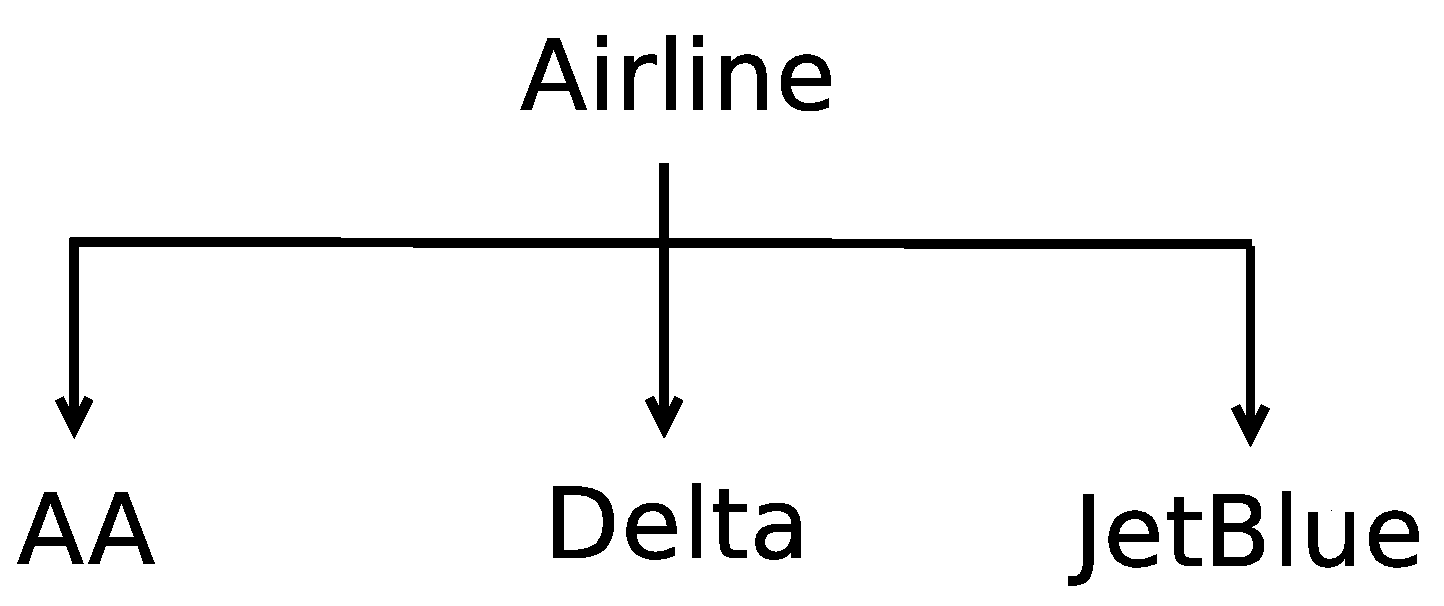
\includegraphics[width=0.35\columnwidth]{drawing/two-level.eps}
\caption{A two-level query facet for the query ``baggage allowance''}
\label{fig:bg-2level}
\end{figure}
When there are only two levels in a query facet, we can call the parent node (or more precisely, its presentation term) \textbf{facet label} (\eg, \concept{airline}), and the child nodes \textbf{facet terms} (\eg, \concept{AA}, \concept{Delta}, \concept{JetBlue}). 
Because all the facet terms are directly subsumed by the facet label (by the definition of taxonomy), facet terms essentially are instances of the same semantic class or category (\ie, the semantic class represented by their parent node). From a user's perspective, the facet terms succinctly represent different options in the same category (represented by the facet label) that a user can select to refine the issued query.

Our work generates one-level query facets. A one-level query facet is simply a two-level query facet with the facet label omitted (or missing). In other words, a one-level query facet is a set of facet terms (\eg, \{\concept{AA}, \concept{Delta}, \concept{JetBlue}\}) without a facet label (\eg, \concept{airline}). But as in a two-level query facet, facet terms in a one-level query facet are subsumed by the \textit{missing} facet label, or equivalently they are instances of the same semantic class represented by the \textit{missing} facet label.

\section{Other Related Techniques}
\label{sec:bg-others}
There are a number of techniques developed to achieve similar goals as faceted search or faceted web search. In this section, we discuss query subtopic mining, search result diversification, search result clustering/organization, query suggestion and semantic class extraction.

\subsection{Query Subtopic Mining}
To address multi-faceted queries, much previous work studied mining query subtopics (or aspects). A query subtopic is often defined as a distinct information need relevant to the original query. It can be represented as a set of terms that together describe the distinct information need~\cite{wang2009mining,wu2011identifying, dang2011inferring} or as a single keyword that succinctly describes the topic~\cite{song2011overview}. For example, \{\concept{news}, \concept{cnn}, \concept{latest news}, \concept{mars curiosity news}\} is a query subtopic for the query \textit{mars landing}, which describes the search intent of Mars landing news. \{\concept{photos}, \concept{NASA}, \concept{new photos}, \concept{curiosity rover photos}\} is another query subtopic for the query, which describes the search intent about Mars landing photos.

Different resources have been used for mining query subtopics. \citet{wang2007learn} and \citet{hu2012mining} used related queries from search logs as candidates, and clustered them into query subtopics. \citet{wang2007learn}, for example, used snippets of a query's clicked web documents to enrich the query representation, and then cluster related past queries into query subtopics.
Due to data sparsity for instance-level query subtopics, some work~\cite{wang2009mining,xue2011topic,wu2011identifying,yin2010building} mined generic query subtopics, which are query subtopics for a generic class of queries. For example, \citet{yin2010building} built taxonomies of query subtopics for categories of name entity queries using search logs. \citet{wu2011identifying} also worked on identifying query aspects for named entities queries. They propagated reformulation phrases for a classes of named entities queries. Other than query logs, query subtopics can also be mined from documents. For example, \citet{dang2011inferring} worked on clustering related anchor texts in ClueWeb09 corpus into query subtopics. \citet{allan2002using}, from a text corpus, extracted commonly occurring parts of speech pattern near a single-word query to find different potential specifications of the query.
\todo{top ranked documents}

Query subtopics and facets are different in that the terms in a query subtopic are not restricted to have any specific semantic relations or structures. However, the terms (more precisely the concepts) in a facet are organized in the taxonomy tree, and they need to subsume its child terms in the tree. For example, the query subtopic \{\concept{news}, \concept{cnn}, \concept{latest news}, \concept{mars curiosity news}\} describes the search intent of Mars landing news, but there are no specific semantic relations between the terms in it, and thus it is not a facet. Instead, a valid facet that describes Mars landing news could be nodes \concept{cnn}, \concept{abc}, \concept{fox} with a parent node \concept{news channels}, where the parent node \concept{new channels} subsumes all the child nodes by the IS-A relations between them. Note that the parent node can be omitted, in the case of one-level facet (See Section~\ref{sec:bg-fws}).
%In a recent work~\cite{Dou:2011:FDQ:2063576.2063767}, Dou et al. developed a system to extract facets from web search results and showed the potential of doing so. However, the unsupervised method they proposed is far from optimal, and it does not improve by having human labels available. Also, to the best of our knowledge, their evaluation can be problematic in some cases, which will be discussed in Section~\ref{sec:evalmetricsall}.

\subsection{Search Results Diversification}
Search result diversification has been studied as a method of tackling ambiguous or multi-faceted queries, while a ranked list of documents remains the primary output feature of Web search engine today. The purpose is to diversify the ranked list to account for different search intents or query subtopics.
%~\cite{clarke2008novelty,sakai2011evaluating}
Techniques studied for search result diversification can be classified by whether or not they explicitly represent the query subtopics in their models. As a result, they are often
categorized as being implicit or explicit. 

Implicit approaches~\cite{carbonell1998use,zhai2003beyond} try to select documents that are different to the previously selected documents to reduce redundancy or increase novelty, without explicitly modeling the actual subtopics. For example, the pioneer implicit approach is known as Maximal Marginal Relevance~\cite{carbonell1998use}. This technique was originally proposed to reduce redundancy in document rankings as well as in text summarization. It scores each candidate document by its estimated relevance to the search query discounted by its maximum similarity with respect to the documents that have been selected earlier. Then it uses a greedy algorithm to select/rank documents based on the scores, as exact maximizing the diversification objective is NP-hard.

Explicit  approaches~\cite{agrawal2009diversifying,carterette2009probabilistic,santos2010exploiting,dang2012diversity,dang2013term}, instead, model query subtopics explicitly and the directly select documents that cover different subtopics. For example, \citet{agrawal2009diversifying} used the Open Directory Project taxonomy to model
query subtopics. Queries are classified into categories (nodes) in the taxonomy, and these categories are used as query subtopics. Then, documents are favored if they are classified into the categories that are less-represented by the documents that have been selected earlier. \citet{santos2010exploiting} used a similar diversification model. The difference between them is: \citet{agrawal2009diversifying} used the Open Directory Project taxonomy to represent query subtopics, while \citet{santos2010exploiting} used the query suggestions obtained from commercial search engines for each query as its query subtopics. 
 
Search result diversification could increase the likelihood that users will
find documents relevant to their specific search intent. However, a weakness of this technique is that the query subtopics are hidden from the user, leaving him or her to guess at how the results are organized. Faceted Web Search addresses this problem by explicitly presenting different facets of a query for users to select.
\todo{difference}

\subsection{Search Result Clustering and Organization}
Search result clustering is a technique that organizes search results by grouping them into, usually labeled, clusters by query subtopics~\cite{cutting1992scatter,kaki2005findex,zamir1999grouper,carpineto2009survey}. It not only offers a complementary view to the flat ranked list of search results, but also provide users the ability to choose the clusters of interest in an interactive manner. An extensive survey for search result clustering is provided by \citet{carpineto2009survey}. In the following, we provide a brief discussion for several prominent search result clustering systems.

Scatter/Gather~\cite{cutting1992scatter,hearst1996reexamining} is an landmark example of search result clustering systems. The system clusters documents into a set of groups, and each group is labeled with a few most frequently occurring words in the cluster's documents. Then a user is expected to select one or two clusters which are thought to contain the documents of interest. After that the selected groups are re-clustered and again labeled. The user can continues this process of drilling down until a satisfactory group of documents is gathered.

One major limitation in Scatter/Gather is the generated cluster labels can be difficult for users to interpret. The labels are simply sets of frequently occurring words, and thus they may not be meaningful to the users. \citet{zamir1999grouper,zamir1998web} addressed the problem by using phrases that appear frequently in the clustered documents as labels. To support online processing, they developed the Suffix Tree Clustering algorithm for clustering and identifying phrase labels efficiently.

In addition to research projects, search result clustering is also used in commerce search engines. The first commercial application is probably Northern Light in the end of the 1990s. The system is based on a set of predefined categories for web documents, and search results are clustered by their categories. After Northern Light, a major breakthrough was made by Vivisimo, which generates clusters and cluster labels for search results dynamically. 

%Most previous work has exploited different textual features extracted from the input texts and applied different clustering algorithms with them.

Instead of organizing search results in groups, there is also some work~\cite{lawrie2001finding,lawrie2003generating, nevill1999lexically} that summarizes search results or a collection of documents in a topic hierarchy. For example, previous studies~\cite{lawrie2001finding,lawrie2003generating} used a probabilistic model for creating topical hierarchies, in which a graph is constructed based on conditional probabilities of words, and the topic words are found by approximately maximizing the predictive power and coverage of the vocabulary.


Faceted Web Search is different from these work in that it provides facets of a query, instead of directly organizing the search results. The facet interface allows users to filter/re-rank search results from multiple aspects, instead of a single taxonomic order. The utility of faceted search interface was investigated in various studies~\cite{pollitt1998key,hearst2006clustering,pratt1999knowledge,yee2003faceted,kaki2005findex,rodden2001does}, where it was shown that users engaged in exploratory tasks often prefer the faceted search interface over simple ranked result list, as well as the alternative ways of organizing search results.

\subsection{Query Suggestion}
Query suggestion (or query recommendation) is a common technique used by search engines to assist users in reformulating queries. In the suggestion process, a user start with issuing an initial query that may be ineffective. Then, the system provides a set of alternative queries that may better address the user's information need as suggestions. After that, the user can select one of the query suggestion to search again. We show an example in Figure~\ref{fig:bg-qsuggestion}, in which a list of related queries for the query \concept{baggage allowance} are suggested.  

\vspace{+5mm}
\begin{figure}[!htbp]
\centering
\includegraphics[width=0.5\columnwidth]{figure2/query-suggestion.png}
\caption{Example query suggestions for the query \concept{baggage allowance}}
\label{fig:bg-qsuggestion}
\end{figure}

Query suggestion and Faceted Web Search are similar in that both of them provide terms for users to select and reformulate queries. However, they are very different in the philosophy behind. In query suggestion, the system provides related queries or queries similar to the initial issued query, and the provided suggestions are used to replace the initial query. In Faceted Web Search, the system provides facets for the query, which describe the search intent from different aspects and are used to refine the initial query instead of replacing it. Due to the difference in the philosophy behind, the way they present suggestions/facet terms are very different. Query suggestions are presented (usually) as a flat list, as shown in Figure~\ref{fig:bg-qsuggestion}. Faceted Web Search instead presents facet terms in a more structured way. The facet terms are grouped together in query facets. For example, in Figure~\ref{fig:fws-example}, \concept{AA}, \concept{Delta}, \concept{JetBlue} are grouped together under \concept{Airline}. By grouping terms into query facets, the facet interface essentially provides a skip list of these facet terms for users. More specifically, a user can skip an entire query facet if the user finds the facet irrelevant, while in the query suggestion interface, the user need to examine each suggestions one by one.


There has been significant previous work on query suggestion, we briefly review some of it below. Most of the previous work relies on query logs for query suggestion~\cite{baeza2004query,jones2006generating,mei2008query,ozertem2011suggestion}. For example, \citet{baeza2004query} provided query suggestions by clustering related queries in query logs, and \citet{jones2006generating} suggested strongly related queries identified from pairs of successively issued queries found in query logs. One widely used technique is exploiting query-click graphs~\cite{craswell2007random,mei2008query,ozertem2011suggestion}. The query-click graph~\cite{craswell2007random} is a bipartite graph consists of nodes representing queries and documents. The two types of nodes are connecting by edges representing clicks on the document for that query. By performing a random walking on this bipartite graph, query similarity can be calculated, and more similar queries can be shown as suggestions. 

In the cases where query logs are not available, only a few methods have been proposed for query suggestions. \citet{bhatia2011query} relied on the corpus to find related queries as suggestions. They extracted frequently occurring phrases and n-grams from the text corpus, and used them as suggestions for auto-completing the query that a user is typing.  \citet{luo2008medsearch} relied on MeSH (Medical Subject Headings), a medical thesaurus, to find related medical phrases as query suggestions for a medical search engine.

%Another line of related work on query suggestion is diversifying query suggestions (e.g., [73, 94]). While search result diversification (e.g., [3, 18]) aims at producing retrieval results that contain a mixture of (topically) different documents, query-side diversification focuses on generating a list of diverse queries, which maximizes the diversity between query-suggestion pairs. 
%Ma et al. [73] proposed a framework for diversifying query suggestions. They first generated the Markov random walk model on the query-URL bipartite graph by adding the top ranked query into a candidate set. Then, other queries were ranked by running the expected hitting time analysis, which could demote the ranks of (unranked) queries to the ranked queries. Thus, the result of ranked suggestions (i.e., queries) could be diversified. 
%Song et al. [94] also discussed the same problem, and selected query candidates from query logs by ranking them in the order that maximizes the similarity and diversity between the queries.
% They measures diversity based on the difference between the original search results and the results of suggested queries. To quantify the difference, several features were devised, e.g., the similarity of the ODP3 category of two search results, rank correlation coefficient for the URLs in two search results, etc. However, these studies are also limited in their application to domain-specific search environments as they require query logs and clickthrough statistics.


\subsection{Semantic Class Extraction}
Semantic class extraction is to automatically mine semantic classes represented as their class instances from certain data corpora. For example, it may extract \textit{USA}, \textit{UK}, \textit{China} as class instances of semantic class \textit{country}. Due to the similar semantic relationships between terms inside a facet and a semantic class, semantic class extraction can be used for facet generation. 

Existing approaches can be roughly divided into two categories: distributional similarity and pattern-based~\cite{shi2010corpus}. The distributional similarity approach is based on the distributional hypothesis~\cite{Harris}, that terms occurring in analogous contexts tend to be similar. Different types of contexts have been studied for this problem, including syntactic context~\cite{lin1998automatic,pantel2002discovering} and lexical context~\cite{pantel2004towards,agirre2009study,pantel2009web}. \citet{lin1998automatic} constructed syntactic context using dependency triples extracted from text corpus. A dependency triple consist of two words and the grammatical relationship between them in the input sentences. The dependency triples are aggregated as syntactic context for each words. The construction of syntactic contexts requires sentences to be parsed by a dependency parser, which may be extremely time-consuming on large corpora. As an alternative, lexical context can be constructed much efficiently. For 
example, \citet{agirre2009study} simply constructed lexical context by using the the surrounding words in sentences. Based on the context representation, clustering algorithms can be applied to cluster similar words/phrases together as a semantic class~\cite{pantel2002discovering}.


The pattern-based approach applies textual patterns~\cite{hearst1992automatic,pasca2004acquisition}, HTML patterns~\cite{shinzato2005simple} or both~\cite{zhang2009employing,shi2010corpus} to extract instances of a semantic class from some corpus. For example, \citet{hearst1992automatic} used pattern \concept{NP such as NP, NP…, and NP} to extract hyponyms and hypernyms, where the hyponyms can be used as candidates for semantic class instances. \citet{shinzato2005simple} used patterns to extract HTML itemized-lits as semantic class. Our work use both types of extraction patterns for facet generation, and they are discussed in details in Section~\ref{sec:facet-candidate}. The raw semantic class extracted can be noisy. To address this problem, \citet{zhang2009employing} used topic modeling to refine the extracted semantic classes. Their assumption is that, like documents in the conventional setting, raw semantic classes are generated by a mixture of hidden semantic classes.

In this work, we apply pattern-based semantic class extraction on the top search results to extract candidates for facet generation (Section~\ref{sec:facet-candidate}), and design some features based on distributional similarity for refining facet candidates (Section~\ref{sec:facet-features}).


%\section{User Feedback}
%There is a long history of using user explicit feedback to improve retrieval performance. In relevance feedback~\cite{rocchio71relevance,salton90improvingretrieval}, documents are presented to users for judgment, after which terms are extracted from the judged relevant document, and added into the retrieval model. In the case where true relevance judgments are unavailable, top documents are assumed to be relevant, which is called pseudo relevance feedback~\cite{buckley1995automatic,abdul2004umass}. Because a document is a large text unit which can be difficult for users to judge and for the system to incorporate relevance information, previous work also studied user feedback on passages~\cite{allan1995relevance,xu1996query} and terms~\cite{koenemann1996case,tan2007term}.

%For faceted search, previous work~\cite{zhang2010interactive} studied user feedback on facets, using both boolean filtering and soft ranking models. However, the study is based on corpora with human created facet metadata, which is difficult to obtain for the general web. One other difference between our work and most other user feedback work is, facet feedback in our work is used to improve ranking with respect to the query subtopic specified by the feedback terms, instead of the query topic represented by the original query. This presents the scenario in Faceted Web Search, where users start with a less-specified query, and then use facets to help clarify and search for subtopic information.

\section{Summary}
Faceted search is the combination of directed search and faceted navigation which enables users to search and navigate through a multi-dimensional information space. Faceted navigation is based on a faceted taxonomy consists of a set of independent taxonomies (called facets) to be combined for expressing compound information needs. Faceted Web Search, the focus of this work, is the extension of faceted search to the open-domain web setting. In our work, we direct extract facets for queries from search results, called \concept{query facets}. For two-level query facets, we call the parent node \concept{facet label}, and the child node \concept{facet terms}. As a start for Faceted Web Search, this work focuses on studying one-level facets, which consist of only facet terms with no facet labels.

Faceted Web Search we propose in this work is different from all the past work. It extends conventional faceted search from a fixed-domain setting to an open-domain web setting. It is different from search result diversification in that instead of hiding those query subtopics from users, it explicitly presents different facets of a query. It is also different from search results clustering or organization in that instead of directly organizing the search results, the facet interface in Faceted Web Search allows users to filter/re-rank search results from multiple aspects.

We study three main issues of Faceted Web Search that have not been explored in previous work, including facet generation, facet feedback and evaluation for Faceted Web Search. Facet generation for Faceted Web Search is different from query subtopic mining because of the different nature of query subtopics and query facets. It is also different from semantic class extraction in that it targets a general web query instead of a semantic class. Facet feedback for Faceted Web Search is different from other user feedback because of their different purposes (discussed in Section~\ref{sec:feedback-related}). 
%Facet feedback targets at improving ranking with respect to the ``query subtopic'' specified by the feedback terms, instead of the query topic represented by the original query.
Our evaluation for Faceted Web Search is also different from previous ones for faceted search in that we do not rely on expensive user studies, and thus our evaluating methods are relative cheap to extend for evaluating new systems.